\documentclass[12pt]{article}

\setlength{\oddsidemargin}{0.5in} \setlength{\evensidemargin}{1in}
\setlength{\textwidth}{6.0in}   \setlength{\headsep}{0.3in}
\setlength{\parindent}{0.2in}   \setlength{\topmargin}{0.0in}
\setlength{\voffset}{-0.3in}    \setlength{\hoffset}{-0.3in}
\setlength{\textheight}{9.2in}  \setlength{\footskip}{0.3in}

\usepackage{amsmath, amsfonts, latexsym, amsthm, amssymb}
\usepackage{graphicx}
\usepackage{chicago,setspace,color}
\usepackage{multirow}

%\newcommand{\Deltahat}    {\hat{\mbox{\bf Delta}}}
%\doublespacing




%  Figure commands for postscript files (.ps)

%  For usual case

%\newcommand{\psfig}[3]{
%  \begin{figure}
%    \vspace{4in}
%    \begin{picture}(0,0)
%      \put(60.,-40.){
%        \special{psfile=figs/#1 hscale=45 vscale=40}
%      }
%    \end{picture}
%    \caption[#2}
%    \label{#3}
%  \end{figure}
%}

%  This is a version of psfigb for two-panel figures

%\newcommand{\psfigbtwo}[3]{
%  \begin{figure}
%    \vspace{3.0in}
%    \begin{picture}(0,0)
%      \put(-103.,-180.)
%        {\special{psfile=figs/#1 hscale=94 vscale=68}}
%  \end{picture}
%  \caption[#2}
%  \label{#3}
%  \end{figure}
%}
%
%%  This is for the first two lupus figures
%
%\newcommand{\psfiglup}[3]{
%  \begin{figure}
%    \vspace{3.0in}
%    \begin{picture}(0,0)
%      \put(-30.,-105.){
%        \special{psfile=figs/#1 hscale=68 vscale=50}
%      }
%    \end{picture}
%    \caption[#2}
%    \label{#3}
%  \end{figure}
%}

% This leaves a bit more space at the bottom
%\newcommand{\psfigg}[3]{ \begin{figure} \vspace{2.9in}
%                       \begin{picture}(0,0) \put(10.,-80.)
%                            {\special{psfile=figs/#1
%                               hscale=47 vscale=47}} \end{picture}
%                       \caption[#2} \label{#3} \end{figure} }
%
%%  This for leaving space for a figure
%\newcommand{\psfiga}[2]{ \begin{figure} \vspace{2.92in}
%\caption[#2} \label{fig:#1} \end{figure}}
%
%%  This uses same string for file name and label
%\newcommand{\psfigb}[2]{ \begin{figure} \vspace{2.92in}
%\begin{picture}(0,0)
%\put(0.,-100.)
%   {\special{psfile=
%       figs/#1.ps
%      hscale=50 vscale=50}}
%\end{picture}
%\caption[#2} \label{fig:#1} \end{figure}}

%  This puts the figure a bit higher up to make some more space
%\newcommand{\psfigbb}[2]{ \begin{figure} \vspace{2.9in}
%\begin{picture}(0,0)
%\put(10.,-80.)
%   {\special{psfile=
%       figs/#1.ps
%      hscale=47 vscale=47}}
%\end{picture}
%\caption[#2} \label{fig:#1} \end{figure}}
%
%%  This is a little one..
%\newcommand{\psfigbshort}[2]{ \begin{figure} \vspace{2.5in}
%\begin{picture}(0,0)
%\put(0.,-90.)
%   {\special{psfile=figs.dir/#1.ps
%      hscale=45 vscale=45}}
%\end{picture}
%\caption[#2} \label{fig:#1} \end{figure}}
%
%
%%  Figure commands for encapsulated postscript files (.eps)
%
%\newcommand{\putfig}[3][8cm]{
%\begin{figure}  \centering \leavevmode
%  \epsfig{file=CSTR/figs/#1,silent=,height=50}
%\caption[#2} \label{#3}
%\end{figure}
%}
%
%%
%%  Inner product macro
%%
%\newcommand{\IP}[2]{ \langle #1 , #2 \rangle }
%\newcommand{\IPvec}[2]{ #1' #2  }
%
%%
%\newcommand{\twobytwo}[4]{\left ( \begin{array}{cc}#1&#2\\#3&#4 \end{array}
%\right ) }
%\newcommand{\twobyone}[2]{\left ( \begin{array}{c}#1 \\ #2 \end{array}
%\right ) }
%\newcommand{\twobytwob}[4]{\left [ \! \begin{array}{cc}#1&#2\\#3&#4 \end{array}
%\! \right ] }
%\newcommand{\twobyoneb}[2]{\left [\! \begin{array}{c}#1 \\ #2 \end{array}
%\! \right ] }
%\renewcommand{\ne}{\! \not \, = }
%%\newcommand{\be}[1]{\begin{equation}\label{#1}}
%\newcommand{\ee}{\end{equation}}
\newcommand{\cJ}{{\mathcal J}}
\newcommand{\cK}{{\mathcal K}}
%\newcommand{\cS}{{\mathcal S}}
%\newcommand{\cT}{{\mathcal T}}
%\newcommand{\cV}{{\mathcal V}}
%\newcommand{\cZ}{{\mathcal Z}}
%\newcommand{\muh}{\hat{\mu}}
%\newcommand{\Gamh}{\hat{\Gamma}}
%\newcommand{\gamh}{\hat{\gamma}}
%\newcommand{\gamt}{\tilde{\gamma}}
%\newcommand{\xit}{\tilde{\xi}}
%\newcommand{\ut}{\tilde{u}}
%\newcommand{\vt}{\tilde{v}}
%\newcommand{\lamh}{\hat{\lambda}}
\newcommand{\gamb}{\mbox{\boldmath$\gamma$}}
\newcommand{\Gamb}{\mbox{\boldmath$\Gamma$}}
\newcommand{\betb}{\mbox{\boldmath$\beta$}}
%\newcommand{\bX}{{\bf X}}
%\newcommand{\bg}{{\bf g}}

\newcommand{\Normal}   {\mbox{\tt Normal}}
\newcommand{\ROUPEN}   {\mbox{\tt ROUPEN}}
\newcommand{\PEN}      {\mbox{\tt PEN}}
\newcommand{\PENRSS}   {\mbox{\tt PENRSS}}
\newcommand{\REGSSE}   {\mbox{\tt REGSSE}}
\newcommand{\PCASSE}   {\mbox{\tt PCASSE}}
\newcommand{\PCAPSV}   {\mbox{\tt PCAPSV}}
\newcommand{\LMSSE}    {\mbox{\tt LMSSE}}
\newcommand{\PENSSE}   {\mbox{\tt PENSSE}}
\newcommand{\SMPENSSE} {\mbox{\tt SMPENSSE}}
\newcommand{\LIK}      {\mbox{\tt LIK}}
\newcommand{\PENLIK}   {\mbox{\tt PENLIK}}
\newcommand{\PROFSSE}  {\mbox{\tt PROFSSE}}
\newcommand{\RSQ}      {\mbox{\tt RSQ}}
\newcommand{\FRATIO}   {\mbox{\tt FRATIO}}
\newcommand{\SMSSE}    {\mbox{\tt SMSSE}}
\newcommand{\LOCSSE}   {\mbox{\tt SMLOCSSE}}
\newcommand{\Kern}     {\mbox{\tt Kern}}
\newcommand{\Triang}   {\mbox{\tt Triang}}
\newcommand{\cov}      {\mbox{\tt cov}}
\newcommand{\corr}     {\mbox{\tt corr}}
\newcommand{\var}      {\mbox{\tt var}}
\newcommand{\SD}      {\mbox{\tt SD}}
\newcommand{\GCV}      {\mbox{\tt GCV}}
\newcommand{\GACV}      {\mbox{\tt GACV}}
\newcommand{\AIC}      {\mbox{\tt AIC}}
\newcommand{\CV}       {\mbox{\tt CV}}
\newcommand{\DF}       {\mbox{\tt DF}}
\newcommand{\LMISE}    {\mbox{\tt LMISE}}
\newcommand{\GFR}      {{\tt GFR}}
\newcommand{\GOP}      {{\tt GOP}}
\newcommand{\KUC}      {{\tt KUC}}

\newcommand{\Height}   {\mbox{\tt Height}}
\newcommand{\Temp}     {\mbox{\tt Temp}}
\newcommand{\TempRes}  {\mbox{\tt TempRes}}
\newcommand{\Prec}     {\mbox{\tt Prec}}
\newcommand{\LogPrec}  {\mbox{\tt LogPrec}}
\newcommand{\LogPrecRes}  {\mbox{\tt LogPrecRes}}
\newcommand{\Precmn}   {\mbox{\tt Precmn}}
\newcommand{\Prectot}  {\mbox{\tt Prectot}}
\newcommand{\Precstar} {\mbox{{\tt Prec}^{*}}}
\newcommand{\LPrec}    {\mbox{\tt LPrec}}
\newcommand{\Hip}      {\mbox{\tt Hip}}
\newcommand{\Knee}     {\mbox{\tt Knee}}
\newcommand{\Hipmn}    {\mbox{\tt Hipmn}}
\newcommand{\Kneemn}   {\mbox{\tt Kneemn}}
\newcommand{\Angles}   {\mbox{\tt Angles}}
\newcommand{\ScriptX}  {\mbox{\tt ScriptX}}
\newcommand{\ScriptY}  {\mbox{\tt ScriptY}}
\newcommand{\GDP}      {\mbox{\tt GDP}}
\newcommand{\Tray}     {\mbox{\tt Tray}}
\newcommand{\DTray}    {\mbox{\tt DTray}}
\newcommand{\Reflux}   {\mbox{\tt Reflux}}
\newcommand{\MSE}      {\mbox{\tt MSE}}
\newcommand{\EMSE}      {\mbox{\tt EMSE}}
\newcommand{\IMSE}     {\mbox{\tt IMSE}}
\newcommand{\RMSE}     {\mbox{\tt RMSE}}
\newcommand{\Bias}     {\mbox{\tt Bias}}
\newcommand{\Var}      {\mbox{\tt Var}}
\newcommand{\STD}      {\mbox{\tt STD}}
\newcommand{\MAD}      {\mbox{\tt MAD}}
\newcommand{\median}      {\mbox{\tt median}}
\newcommand{\E}      {\mbox{\tt E}}
\newcommand{\tr}      {\mbox{\tt Tr}}
\newcommand{\Stt}      {\mbox{\tt S}}
\newcommand{\Ctt}      {\mbox{\tt C}}
\newcommand{\SSE}      {\mbox{\tt SSE}}
\newcommand{\WSSE}      {\mbox{\tt WSSE}}
\newcommand{\TPE}      {\mbox{\tt TPE}}
\newcommand{\SSY}      {\mbox{\tt SSY}}
\newcommand{\PSSE}     {\mbox{\tt PSSE}}
\newcommand{\MSR}      {\mbox{\tt MSR}}
\newcommand{\tPDA}     {\mbox{\tiny PDA}}
\newcommand{\tPCA}     {\mbox{\tiny PCA}}
\newcommand{\Force}    {\mbox{\tt Force}}
\newcommand{\ForceX}   {\mbox{\tt ForceX}}
\newcommand{\ForceY}   {\mbox{\tt ForceY}}
\newcommand{\Contrast} {\mbox{\tt Contrast}}
\newcommand{\ytocMap}   {\mbox{\tt y2cMap}}
\newcommand{\YtoCMap}   {\mbox{\tt Y2CMap}}
\newcommand{\ytobMap}   {\mbox{\tt y2bMap}}
\newcommand{\YtoBMap}   {\mbox{\tt Y2BMap}}
\newcommand{\ctorMap}   {\mbox{\tt c2rMap}}
\newcommand{\CtoRMap}   {\mbox{\tt C2RMap}}
\newcommand{\ytorMap}   {\mbox{\tt y2rMap}}
\newcommand{\YtoRMap}   {\mbox{\tt Y2RMap}}
\newcommand{\btorMap}   {\mbox{\tt b2rMap}}
\newcommand{\BtoRMap}   {\mbox{\tt B2RMap}}
\newcommand{\ctobMap}   {\mbox{\tt c2bMap}}
\newcommand{\CtoBMap}   {\mbox{\tt C2BMap}}
\newcommand{\Modulus}   {\mbox{\tt Mod}}
\newcommand{\Phase}     {\mbox{\tt Phase}}
\newcommand{\Probe}     {\mbox{\tt Probe}}
\newcommand{\MINEIG}    {\mbox{\tt MINEIG}}
\newcommand{\dfe}       {\mbox{\tt dfe}}


\newcommand{\Hi}        {\mbox{\footnotesize \tt H}}
\newcommand{\Kn}        {\mbox{\footnotesize \tt K}}
\newcommand{\Hipsmall}  {\mbox{\footnotesize \tt Hip}}
\newcommand{\Kneesmall} {\mbox{\footnotesize \tt Knee}}

\newcommand{\chat}     {\hat{c}}
\newcommand{\dhat}     {\hat{d}}
\newcommand{\ehat}     {\hat{e}}
\newcommand{\fhat}     {\hat{f}}
\newcommand{\rhat}     {\hat{r}}
\newcommand{\uhat}     {\hat{u}}
\newcommand{\vhat}     {\hat{v}}
\newcommand{\xhat}     {\hat{x}}
\newcommand{\yhat}     {\mbox{$\hat{y}$}}
\newcommand{\Fhat}     {\hat{F}}
\newcommand{\Mhat}     {\hat{M}}
\newcommand{\alphahat} {\hat{\alpha}}
\newcommand{\betahat}  {\hat{\beta}}
\newcommand{\thetahat} {\hat{\theta}}

\newcommand{\xtilde}   {\tilde{x}}
\newcommand{\etilde}   {\tilde{e}}
\newcommand{\ktilde}   {\tilde{k}}

\newcommand{\lcal}     {\ell}
\newcommand{\Bcal}     {\mbox{$\cal B$}}
\newcommand{\Fcal}     {\mbox{$\cal F$}}
\newcommand{\Gcal}     {\mbox{$\cal G$}}
\newcommand{\Hcal}     {\mbox{$\cal H$}}
\newcommand{\Lcal}     {\mbox{$\cal L$}}
\newcommand{\Pcal}     {\mbox{$\cal P$}}
\newcommand{\Rcal}     {\mbox{$\cal R$}}
\newcommand{\Scal}     {\mbox{$\cal S$}}
\newcommand{\Tcal}     {\mbox{$\cal T$}}
\newcommand{\Ucal}     {\mbox{$\cal U$}}
\newcommand{\Ycal}     {\mbox{$\cal Y$}}

\newcommand{\TcalX}     {{{\cal T}_{\!X}}}
\newcommand{\TcalY}     {{{\cal T}_{\!Y}}}


\newcommand{\spann}    {\mbox{span}}
\newcommand{\diag}     {\mbox{diag}}
\newcommand{\Exp}      {\mbox{E}}

\newcommand{\abold}    {\mbox{\bf a}}
\newcommand{\bbold}    {\mbox{\bf b}}
\newcommand{\cbold}    {\mbox{\bf c}}
\newcommand{\dbold}    {\mbox{\bf d}}
\newcommand{\ebold}    {\mbox{\bf e}}
\newcommand{\fbold}    {\mbox{\bf f}}
\newcommand{\gbold}    {\mbox{\bf g}}
\newcommand{\hbold}    {\mbox{\bf h}}
\newcommand{\kbold}    {\mbox{\bf k}}
\newcommand{\nbold}    {\mbox{\bf n}}
\newcommand{\pbold}    {\mbox{\bf p}}
\newcommand{\rbold}    {\mbox{\bf r}}
\newcommand{\sbold}    {\mbox{\bf s}}
\newcommand{\tbold}    {\mbox{\bf t}}
\newcommand{\ubold}    {\mbox{\bf u}}
\newcommand{\vbold}    {\mbox{\bf v}}
\newcommand{\wbold}    {\mbox{\bf w}}
\newcommand{\xbold}    {\mbox{\bf x}}
\newcommand{\ybold}    {\mbox{\bf y}}
\newcommand{\zbold}    {\mbox{\bf z}}
\newcommand{\Abold}    {\mbox{\bf A}}
\newcommand{\Bbold}    {\mbox{\bf B}}
\newcommand{\Cbold}    {\mbox{\bf C}}
\newcommand{\Dbold}    {\mbox{\bf D}}
\newcommand{\Ebold}    {\mbox{\bf E}}
\newcommand{\Fbold}    {\mbox{\bf F}}
\newcommand{\Gbold}    {\mbox{\bf G}}
\newcommand{\Hbold}    {\mbox{\bf H}}
\newcommand{\Ibold}    {\mbox{\bf I}}
\newcommand{\Jbold}    {\mbox{\bf J}}
\newcommand{\Kbold}    {\mbox{\bf K}}
\newcommand{\Lbold}    {\mbox{\bf L}}
\newcommand{\Mbold}    {\mbox{\bf M}}
\newcommand{\Nbold}    {\mbox{\bf N}}
\newcommand{\Pbold}    {\mbox{\bf P}}
\newcommand{\Qbold}    {\mbox{\bf Q}}
\newcommand{\Rbold}    {\mbox{\bf R}}
\newcommand{\Sbold}    {\mbox{\bf S}}
\newcommand{\Tbold}    {\mbox{\bf T}}
\newcommand{\Ubold}    {\mbox{\bf U}}
\newcommand{\Vbold}    {\mbox{\bf V}}
\newcommand{\Wbold}    {\mbox{\bf W}}
\newcommand{\Xbold}    {\mbox{\bf X}}
\newcommand{\Ybold}    {\mbox{\bf Y}}
\newcommand{\Zbold}    {\mbox{\bf Z}}


\newcommand{\onebold}   {\mbox{\bf 1}}
\newcommand{\zerobold}  {\mbox{\bf 0}}

\newcommand{\chatbold} {\hat{\mbox{\bf c}}}
\newcommand{\dhatbold} {\hat{\mbox{\bf d}}}
\newcommand{\xhatbold} {\hat{\mbox{\bf x}}}
\newcommand{\yhatbold} {\hat{\mbox{\bf y}}}
\newcommand{\Ahatbold} {\hat{\mbox{\bf A}}}
\newcommand{\Bhatbold} {\hat{\mbox{\bf B}}}
\newcommand{\Qhatbold} {\hat{\mbox{\bf Q}}}
\newcommand{\Rhatbold} {\hat{\mbox{\bf R}}}
\newcommand{\Yhatbold} {\hat{\mbox{\bf Y}}}
\newcommand{\Ccal}    {\mathcal{C}}
\newcommand{\Uboldtilde}    {\tilde{\mbox{\bf U}}}
\newcommand{\Zboldtilde}    {\tilde{\mbox{\bf Z}}}
\newcommand{\Dboldtilde}    {\tilde{\mbox{\bf D}}}
\newcommand{\Deltatilde}    {\tilde{\mbox{ {$\Delta$}}}}
%\newcommand{\aboldhat}    {\hat{\mbox{\bf a}}}
\newcommand{\bboldhat}    {\hat{\mbox{\bf b}}}
\newcommand{\cboldhat}    {\hat{\mbox{\bf c}}}
\newcommand{\xboldhat}    {\hat{\mbox{\bf x}}}
\newcommand{\yboldhat}    {\hat{\mbox{\bf y}}}
\newcommand{\Rboldhat}    {\hat{\mbox{\bf R}}}
\newcommand{\Dboldhat}    {\hat{\mbox{\bf D}}}
\newcommand{\Eboldhat}    {\hat{\mbox{\bf E}}}
\newcommand{\Deltahat}    {\hat{\mbox{\Delta}}}

\newcommand{\varphibold}   {\mbox{\boldmath${\varphi}$}}
\newcommand{\alphabold}   {\mbox{\boldmath${\alpha}$}}
\newcommand{\betabold}    {\mbox{\boldmath${\beta}$}}
\newcommand{\epsilonbold} {\mbox{\boldmath${\epsilon}$}}
\newcommand{\etabold}     {\mbox{\boldmath${\eta}$}}
\newcommand{\gammabold}   {\mbox{\boldmath${\gamma}$}}
\newcommand{\lambdabold}  {\mbox{\boldmath${\lambda}$}}
\newcommand{\mubold}      {\mbox{\boldmath${\mu}$}}
\newcommand{\phibold}     {\mbox{\boldmath${\phi}$}}
\newcommand{\Phibold}     {\mbox{\boldmath${\Phi}$}}
\newcommand{\psibold}     {\mbox{\boldmath${\psi}$}}
\newcommand{\Psibold}     {\mbox{\boldmath${\Psi}$}}
\newcommand{\thetabold}   {\mbox{\boldmath${\theta}$}}
\newcommand{\Thetabold}   {\mbox{\boldmath${\Theta}$}}
\newcommand{\Sigmabold}   {\mbox{\boldmath${\Sigma}$}}
\newcommand{\Sigb}        {\mbox{\boldmath${\Sigma}$}}
\newcommand{\xibold}      {\mbox{\boldmath${\xi}$}}
\newcommand{\zetabold}    {\mbox{\boldmath${\zeta}$}}
\newcommand{\trace}    {\mbox{trace}}
\newcommand{\aboldhat} {\hat{\mbox{\boldmath${a}$}}}
% \newcommand{\bboldhat} {\hat{\mbox{\boldmath${b}$}}}
\newcommand{\lambdaboldhat} {\hat{\mbox{\boldmath${\lambda}$}}}
\newcommand{\betaboldhat} {\hat{\mbox{\boldmath${\beta}$}}}
\newcommand{\gammaboldhat} {\hat{\mbox{\boldmath${\gamma}$}}}
\newcommand{\thetaboldhat} {\hat{\mbox{\boldmath${\theta}$}}}
\newcommand{\Sigmaboldhat} {\hat{\mbox{\boldmath${\Sigma}$}}}
\newcommand{\muboldhat} {\hat{\mbox{\boldmath${\mu}$}}}

\newcommand{\xbar}     {\bar{x}}
\newcommand{\ybar}     {\bar{y}}
\newcommand{\Pbar}     {\bar{P}}

\newcommand{\gtilde}       {\tilde{g}}
\newcommand{\ntilde}       {\tilde{n}}
\newcommand{\alphatilde}   {\tilde{\alpha}}
\newcommand{\betatilde}    {\tilde{\beta}}

\newcommand{\dstar}    {d^{*}}
\newcommand{\estar}    {e^{*}}
\newcommand{\fstar}    {f^{*}}
\newcommand{\ustar}    {u^{*}}
\newcommand{\vstar}    {v^{*}}
\newcommand{\xstar}    {x^{*}}
\newcommand{\ystar}    {y^{*}}
\newcommand{\zstar}    {z^{*}}
\newcommand{\Astar}    {A^{*}}
\newcommand{\Bstar}    {B^{*}}
\newcommand{\Estar}    {E^{*}}
\newcommand{\Fstar}    {F^{*}}
\newcommand{\Lstar}    {L^{*}}
\newcommand{\Pstar}    {P^{*}}
\newcommand{\Ustar}    {U^{*}}
\newcommand{\Vstar}    {V^{*}}
\newcommand{\Xstar}    {X^{*}}
\newcommand{\cN}       {\textit{N}}

\newcommand{\eperp}        {e^{\bot}}

\newcommand{\xboldstar}    { {\mbox{\bf x}}^{*}}
\newcommand{\yboldstar}    { {\mbox{\bf y}}^{*}}
\newcommand{\zboldstar}    { {\mbox{\bf z}}^{*}}
\newcommand{\Zboldstar}    { {\mbox{\bf Z}}^{*}}
\newcommand{\Zboldstart}   { {\mbox{\bf Z}}^{*'}}
\newcommand{\ystarhat}     { \hat{y}^{*}}
\newcommand{\yboldstarhat} { \hat{\mbox{\bf y}}^{*}}

\newcommand{\betastar} {\beta^{*}}
\newcommand{\etastar}  {\eta^{*}}

\newcommand{\Pbarstar} {\bar{P}^{*}}

\newcommand{\Aplus}    {A^{+}}

\newcommand{\Amins}    {A^{-}}
\newcommand{\Xmins}    {X^{-}}
\newcommand{\Zmins}    {Z^{-}}

\newcommand{\Zinv}     {Z^{-1}}
\newcommand{\Zginv}    {Z^{-}}


\newcommand{\Zboldinv} {\mbox{\bf Z}^{-1}}

\newcommand{\Qboldginv}{\mbox{\bf Q}^{-}}
\newcommand{\Rboldginv}{\mbox{\bf R}^{-}}
\newcommand{\Zboldginv}{\mbox{\bf Z}^{-}}

\newcommand{\rank}     {\mbox{rank}}
\newcommand{\veccom}   {\mbox{vec}}

\newcommand{\smint}{\! \int \!}
\newcommand{\Gambt}{\tilde{\mbox{\boldmath${\Gamma}$}}}

\newcommand{\cvu}{\mbox{\bf a}}
\newcommand{\cvv}{\mbox{\bf b}}
\newcommand{\cfu}{\mbox{\boldmath${\xi}$}}
\newcommand{\cfv}{\mbox{\boldmath${\eta}$}}
\newcommand{\Vboldt}{\tilde{\Vbold}}
\newcommand{\funcov}{v}
\newcommand{\funcovh}{\hat{v}}
\newcommand{\Funcov}{V}
\newcommand{\Funcovh}{\hat{V}}
\newcommand{\cancov}{{\mbox{\tt ccorsq}}^{pop}}
\newcommand{\cancovh}{\mbox{\tt ccorsq}}

\newcommand{\Splus}{S-PLUS}
\newcommand{\df}{\mbox{\tt df}}
%\newcommand{\etal}{et al.\ }

\newcommand{\pardeltai}  {\frac{\partial  }{\partial \delta_i  } }
\newcommand{\pardeltait} {\frac{\partial^2}{\partial \delta_i^2} }


\newcommand{\argmin}{\ensuremath{\operatornamewithlimits{argmin}}}
\newtheorem{thm}{Theorem}[section]
\newtheorem{lem}[]{Lemma}

\title{Principal Subspace Analysis and Some Extensions Using Parameter Cascading}

\author{J. O. Ramsay and A. Kneip}

% \footnote{James Ramsay is a Professor Emeritus in the Psychology Department at McGill University (Email:  {\tt ramsay@psych.mcgill.ca}) and Alois Kneip is a Professor at the University of Bonn (Email: {\tt akneip@uni-bonn.de})


\begin{document}

\maketitle

\begin{abstract}
\end{abstract}

\textbf{Key Words: marginalization, regularization, nuisance parameters}

%  -----------------------------------------------------------------------------------------------

\section{Introduction}
\label{sec:intro}

This paper investigates the generalization of principal components analysis (PCA) or, more descriptively, \emph{principal subspace analysis}.  A parameter estimation strategy call parameter cascading permits the computation the usual principal components of variation in either a multivariate or functional data context without using eigenanalysis; and, as a consequence, enables a wide range of useful extensions of the classical method.  Among these is an improved version of partial least squares for predicting one or more dependent variables from a reduced rank approximation of the independent variable values, and the registration of functional data to its principal subspace of variation.  

For an $N$ by $n$ multivariate data matrix $\Xbold$, PCA  is its approximation of rank $K$ by the bilinear model $\Fbold \Abold$, where the $N$ by $K$ matrix $\Fbold$ contains in its rows principal component scores for defining the approximation of the data for each case, and the $K$ by $n$ matrix $\Abold$ contains within its columns the principal component coefficients for approximating the variables.  The classical estimation of these matrix parameters can be achieved in one step via the singular value decomposition of $\Xbold$, but computational considerations favour the two-stage process of computing $\Abold$ through the eigenanalysis of $N^{-1} \Xbold' \Xbold = \Vbold \Dbold \Vbold'$, $\Abold'$ being the leading $K$ columns of $\Vbold \Dbold^{1/2}$, and $\Fbold$ defined as 
\begin{equation} \label{Feqtn0}
  \Fbold(\Abold) = \Xbold \Abold' (\Abold \Abold')^{-1}.
\end{equation}
More generally, since it seems to us appropriate to reserve the use of ``principal component'' for the classical estimation of $\Fbold$ and $\Abold$, we refer to these matrix parameters as \emph{factor scores} and \emph{factor loadings}, respectively.  Elsewhere in the mathematical sciences, a plane embedded in higher dimensional Euclidean space is known as a Grassmann manifold.

Why would one want to amend such a well-established and clearly successful statistical method as PCA?  Here are a few of its more serious deficiencies:
\begin{itemize}
  \item  PCA is tightly tied to least squares estimation.  Either the eigenanalysis of $N^{-1}\Xbold'\Xbold$ or the singular value decomposition of $\Xbold$ itself yields a least squares approximation of rank $K$ to the respective matrix by eliminating all but the dominant $K$ eigen- or singular-values, respectively.  However, least squares approximation is often not appropriate; variables like the concentration of a chemical vary between pre-determined limits, other variables are intrinsically non-negative, discrete or even binary, and least squares estimation is problematical in the presence of strongly skewed and long-tailed distributions of residuals in $\Xbold - \Fbold \Abold.$  Consequently the capacity to choose the fitting criterion separately for each variable is likely to improve the quality of what PCA estimates.
  \item  The classical PCA problem is ill-posed.  If order $K$ matrix $\Wbold$ is nonsingular, than PC-scores matrix $\Gbold = \Fbold \Wbold$ and PC-coefficients matrix $\Bbold = \Wbold^{-1} \Abold$ yield the same approximation to the data.  It is well-known in the social science statistical literature that rotations of eigenvectors, where $\Wbold$ is assumed to be orthonormal, can greatly improve the interpretability of the basis for the subspace.  It is easy to see why many well-known texts on multivariate statistics fail to mention this issue; if we assume that the eigenvalues are distinct, then the eigenvector-eigenvalue pairs are uniquely defined.  But as a basis system eigenvectors are merely byproducts of subspace identification, and in no sense are essential to the fundamental PCA problem, which is to define the best-fitting vector subspace of dimension K.  Put another way, eigenvectors over-parameterize the subspace, which, as a Grassmann manifold, is known to have dimension $K(n-K)$ (Boothby, 1975), as opposed to the rank $nK$ of t$\Vbold$.  The PCA problem therefore intrinsically leaves open the question of what basis is used to span the subspace.  Put more succintly, it is the subspace that is the parameter in the PCA model, rather than its particular representation by eigenanalysis.
  \item  Principal component scores and coefficients are treated symmetrically by the singular value decomposition, since it provides essentially the same solution for both $\Xbold$ and $\Xbold'$.  But the dimensions of $\Xbold$ differ in an important way:  the $n$ sets of PC-coefficients in $\Abold$ control the fit to the entire corpus of data,  but each of the $N$ sets of PC-scores, $f_{ik},k=1,\ldots,K$ controls the fit only to the relative small amount of data in the $i$th row of $\Xbold.$  Moreover, $N$ can easily vary greatly from one set of data to another, whereas $n$ is more apt to be considered fixed.  As a consequence, the PC-coefficients are \emph{structural} parameters and the PC-scores are \emph{incidental} or \emph{nuisance} parameters in the terminology of Neyman and Scott (1948), who first showed that the usual estimation methods for structural parameters in the presence of nuisance parameters are neither consistent nor efficient.  The large literature on the nuisance parameter problem has made clear that diffeerent estimation strategies are required for these two parameter classes.
  \item The principle of \emph{regularization} as a means of stabilizing estimates, exchanging squared bias for a reduction in sampling variance, and of incorporating some prior information about what is being estimated is now well established for most popular data analyses, and this also seems desirable for principal components analyses. Moreover, the notion of regularity or smoothness seems likely to differ for factor loadings and factor scores, further emphasizing the need for an asymmetric treatment of the two parameter classes.
  \item It is often essential to fit a model to data by a technique that is robust to outliers.  Indeed, the PCA problem present robustness problems at more levels than that of the residual matrix $\Xbold - \Fbold \Abold$; it is often the case in practice that a principal component emerges early in the sequence that essentially fits a single variable in the multivariate case, or a feature in a single curve in the functional context.  There is already a considerable literature on robust covariance estimation where pure eigenanalysis has to be abandoned to achieve this end.
  \item Interval or confidence region estimation for the eigenvectors requires the assumption of separated eigenvalues, a property that seems artificial in the context of the processes that generate most data.  This highlights the fact that interval estimation for basis systems is the wrong question; what we need is a measure of the sampling variation of the estimated subspace around some ``population'' manifold in frequentist terms, or the posterior probabilities of $K$-dimensional subspaces given $\Xbold$ within a Bayesian framework.
\end{itemize}

Parameter cascading is a strategy for estimating structural parameters $\Abold$ in the presence of nuisance parameters $\Fbold$ by defining the latter as a smooth function $\Fbold(\Abold)$ of the former, with user-control over ``smoothness''.  This functional relationship can often be defined explicitly, but also more generally by specifying an inner data-fitting criterion $G(\Fbold|\Abold)$ that is re-optimized each time there is a change in $\Abold$ during the process of optimizing an outer criterion $H(\Abold)$.  When $H$ and $G$ are the same objective functions, as is the case for the least squares criterion in classical PCA, the use of this functional relationship is the well-known profiling algorithm.  But we argue that there are important reasons for $H$ and $G$ to not to be the same, so that the resulting multi-criterion optimizing parameter cascading strategy is a generalization of profiling.

Parameter cascading was first used by Ramsay, Hooker, Campbell and Cao (2007) for the estimation of parameters defining dynamical systems, a context where an explicit expression of the model is usually not possible.  Cao and Ramsay (2007) and Cao and Ramsay (2008) applied parameter cascading to data smoothing with adaptive regularization in order to adjust confidence intervals to take into account the uncertainty in data-determined smoothing parameters. Cao and Ramsay (2010) used parameter cascading for high-dimensional linear mixed effects models, including those for functional data.  

Parameter cascading is already latent in a wide range of older methodologies, including the use of profiling in nonlinear least squares problems discussed in Bates and Watts (1988) and many other texts, and also in the large literature on the nuisance parameter estimation problem of Neyman and Scott (1948). Parameter cascading is also used in regularized data smoothing and functional parameter estimation in functional data analysis (Ramsay and Silverman, 2005), the REML method for estimating inter-record variance components in random effects models, and some versions of the EM algorithm.

The rest of this paper is organized as follows. Section 2 applies parameter cascading to the estimation of the classical principal components of $\Sbold$, as well as of a set of $N$ observed functions $x_i(t)$ observed over a common domain for continuous index $t$.

%  -----------------------------------------------------------------------------------------------
%  -----------------------------------------------------------------------------------------------

\section{Parameter cascading for Multivariate PCA}
\label{sec:PCforPCA}

We now consider the application of parameter cascading to a variety of types of principal components analyses, including both multivariate and functional versions, partial least squares, and the registration of functional observations to a principal components representation.  For the most part, the path from the multivariate case to other situations is easy to follow, so that we consider parameter cascading for multivariate PCA in some depth.

%  -----------------------------------------------------------------------------------------------

\subsection{Defining the parameter cascaded PCA for multivariate data}
\label{subsec:PCforMPCA}

We define the factor scores in $\Fbold$ as smooth functions of the factor coefficients in $\Abold$; that is, as $\Fbold(\Abold)$.  In effect, this is already achieved in the classic case by the regression equation (\ref{Feqtn0}), but we now wish to add regularization features to the estimation of both $\Fbold$ and $\Abold,$  as well as the variation of fitting criteria over variables.  Let $g_j$ be a fitting criterion specific to variable $j$, which will often be a negative log likelihood tailored to that variable's known distributional characteristics.  Let $P_F$ be regularization function that quantifies one or more aspects of ``roughness'' in the estimate of $\Fbold$.  The inner fitting criterion will usually, but not inevitably, be
\begin{equation} \label{Geqtn1}
  G(\Fbold|\Abold,\Xbold) = \sum_j^n g_j(\xbold_j, \Fbold \abold_j) + P_F(\Fbold),
\end{equation}
where $\xbold_j$ and $\abold_j$ the $j$th column of $\Xbold$ and $\Abold$, respectively.

Among the obvious choices for the roughness term $P_F$ are the quadratic forms $\lambda_1 \trace(\Fbold \Rbold_1 \Fbold')$, $\lambda_2 \trace(\Fbold' \Rbold_2 \Fbold)$ and $\lambda_{12} \veccom(\Fbold)' \Rbold_{12}\veccom(\Fbold)$ that capture roughness in the rows, columns, and vectorized $\Fbold$, respectively.  The roughness penalty matrices $\Rbold_1 \in \Scal^K$, $\Rbold_2 \in \Scal^N$ and $\Rbold_{12} \in \Scal^{NK}$, where $\Scal^m$ is the space of symmetric semidefinite matrices of order $m$, will often be projectors into the complement of some low-dimensional subspace spanned by the known columns of  a pre-specified matrix $\Zbold$.  For example, $\Rbold_2 = \Ibold_N - \Zbold_2(\Zbold_2' \Zbold_2)^{-1}\Zbold_2'$ measures the extent to which columns of $\Fbold$ lie in the subspace spanned by the columns of $\Zbold_2$ having $N$ rows.  Row-regularization using $\Rbold_1 = \Ibold_K$ can reign in the effects of outlying observations on the subspace identification.  The regularization of $\veccom(\Fbold)$ can be used to specify that entries in the matrix have fixed values, which in turn can imply removing some of the unidentified aspects of $\Abold.$  We can also consider the use of $\Lcal_1$ penalties on $\Fbold$ and/or $\Abold$ in order to induce data-defined sparsity in either matrix.

In the specific case of pure least squares estimation, the minimizer of $G$ when $\lambda_2 = \lambda_{12} = 0$ is a simple modification of (\ref{Feqtn0}):
\begin{equation} \label{Feqtn1}
  \Fbold(\Abold) = \Xbold \Abold'(\Abold \Abold' + \lambda_1 \Rbold)^{-1},
\end{equation}
but for $\lambda_2 > 0$ or $\lambda_{12} = 0$ as
\begin{equation} \label{Feqtn2}
  \Fbold(\Abold) = [\Ibold_N \otimes (\Abold \Abold') + \lambda_1 \Ibold_N \otimes \Rbold_1 + \lambda_2 \Rbold_2 \otimes \Ibold_K  + \lambda_{12} \Rbold_{12}]^{-1} \veccom(\Abold \Xbold')
\end{equation}
where $\Ibold_N$ and $\Ibold_K$ are identity matrices of order $N$ and $K$, respectively and $\veccom(\Abold \Xbold')$ is matrix $\Abold \Xbold'$ written column-wise as a vector.  

Next we define the outer factor coefficient criterion
\begin{equation} \label{Heqtn1}
  H(\Abold) = \sum_j^n h_j[\xbold_j, \Fbold(\Abold) \abold_j]  + P_H(\Abold)
\end{equation}
The options for defining the $\Abold$ regularization term $P_H$ contain quadratic row-, column- and vector-regularization strategies analogous to those defined above for $\Fbold$.  

Even with regularization, it may be that a simple rescaling of $\Abold$ can usually be matched by the inverse scaling of $\Fbold$, and for more stable computation it may be useful to assume the scale restriction
\begin{equation} \label{Ascale}
  \| \Abold \| = \rho.
\end{equation}
The optimization $H$ on the $nK$-hypersphere of radius $\rho$ can be achieved by converting the cartesian coordinates $\veccom(\Abold)$ in $nK$ space to hyperspherical angular coordinates of dimension $nK-1$.  Nevertheless, substantial non-identifiability may remain after the choice of $G$ and $H$, and since the optimum may not be unique, second order optimization methods such as Newton-Raphson may fail.  But quasi-Newton and conjugate gradient methods work fine in our experience, even when the hessian matrices associated with $G$ and $H$ are singular.

Of course, the nice explicit conditional minimization results (\ref{Feqtn1}) and (\ref{Feqtn1}) vanish if something other than least squares criteria are involved in the specification of $G$ and $H$, and in this case parameter cascading requires that $G$ be re-optimized each time $\Abold$ is modified.  Moreover, the gradient of $H$ must take into account that $\Fbold$ is a function of $\Abold$.  That is, the total derivative 
\[
  \frac{d H}{d \Abold} = \frac{\partial H}{\partial \Abold} + \bigg[\frac{\partial H}{\partial \Fbold}\bigg] \bigg[\frac{d \Fbold}{d \Abold}\bigg]
\]
From 
\[
  \frac{d}{d \Abold} \bigg(\frac{J}{\partial \Fbold}\bigg) = 
  \frac{\partial^2 J}{\partial \Abold \partial \Fbold} + \bigg[\frac{\partial^2 J}{\partial^2 \Fbold} \bigg] \bigg[\frac{d \Fbold}{d \Abold}\bigg] = 0
\] 
at the conditional optimum of $J$, and assuming that at that point the hessian matrix is nonsingular, we have that
\[
  \frac{d }{d \Abold} \bigg[\frac{\partial J}{\partial \Fbold }\bigg] = \frac{d \Fbold}{d \Abold} + \bigg[\frac{\partial^2 J}{\partial^2 \Fbold} \bigg]^{-1} \bigg[\frac{d \Fbold}{d \Abold}\bigg] = 0
\]
and we arrive at the result known as the implicit function theorem,
\[
  \frac{d H}{d \Abold} = \frac{\partial H}{\partial \Abold} - \bigg[\frac{\partial H}{\partial \Fbold}\bigg] \bigg[\frac{\partial^2 J}{\partial^2 \Fbold} \bigg]^{-1} \bigg[\frac{d \Fbold}{d \Abold}\bigg].
\]

%  --------------------------------------------------------------------------------------------

\subsection{The evaluation and interpretation of the subspace}
\label{subsec:subspace}

If the $K$ dimensional subspace is the model, and the coordinates in the rows of $\Abold$ are in incidental to how the subspace is identified, then it becomes essential to use only quantities that are invariant with respect to a choice of coordinate system in evaluating the fit of a subspace to a known target, its sampling variance, or arriving at a description or interpretation of what space ``means'' in real-world terms.  Fortunately, appropriate tools are readily at hand.  Canonical correlation assesses the congruence of two subpaces of $\cal{R}^{N}$ by the eigenanalysis of the product $\Pbold_1 \Pbold_2$ of the order $N$ projection matrices that define the image of each column of $\Xbold$ on the respective subspace.  The eigenvalues $\rho_k^2$ by order of size are the squared multiple correlations between the associated pair of canonical variables and, as in PCA, the sum of these eigenvalues is an overall measure relative to $K$ of how closely the two subspaces coincide.  Moreover, the smallest $\rho^2_k$ can be interpreted as the cosine of the smallest angle achievable between two vectors in the respective subspaces.

The interpretation of the subspace is necessarily within the context of the variables associated with the columns $\xbold_j$ of $\Xbold$.  A measure of the extent to which a column $j$ is representable within the subspace is
\begin{equation} \label{hdef}
  h_j^2 = \frac{\| \Pbold \xbold_j \|^2 }{ \| \xbold\|^2 }
\end{equation}
where $\Pbold = \Fbold (\Fbold'\Fbold)^{-1} \Fbold'$ projects an $N$-vector on to the subspace.  Squared multiple correlation measure $h_j^2$ is called the ``communality'' of the variable in the social science literature.  A good description of a subspace will choose terms that take account of communalities that are near zero as well as those near one.

%  --------------------------------------------------------------------------------------------

\subsection{An illustration of cascaded multivariate PCA}
\label{subsec:PCMPCAexample}

Figure \ref{MDA1} illustrates the use of this regularization framework for an artificial problem with $N = 200, n = 5$ and $K = 2.$.  The true factor scores in $\Fbold_{pop}$ were $200$ equally spaced points on a circle of unit radius, the $5$ true factor loadings in the first row of $\Abold_{pop}$ were all one, and the loadings in its second row were (-2,-1,0,1,2).  The data matrix was constructed by adding random normally distributed errors to $\Xbold_{pop} = \Fbold_{pop} \Abold_{pop}$ with mean zero and standard deviation 0.5.  The left panel of Figure \ref{MDA1} shows the estimated and true factor scores using least squares criteria for an analysis with no regularization on either $\Fbold$ or $\Abold$ but with the norm constraint (\ref{Ascale}) on $\Abold.$  The error in the data results in factor scores having a roughly elliptical distribution.  Using canonical correlation analysis to measure the agreement between the estimated and true $\Abold$'s results in squared canonical correlations $\rho_1^2 = 0.99991$ and $\rho_2^2 = 0.99775$, indicating an excellent level of agreement between the estimated and true two-dimensional subspaces. That is, although the estimated $\Abold$ differs substantially from its true counterpart, its rows span almost exactly the same subspace.

%%%%%%%%%%%%%%%%%%%%%%%%%%%%%%%%%%%%%%%%%%%%%%%%%%%%%%%%%%%%%%%%%
\begin{figure}
  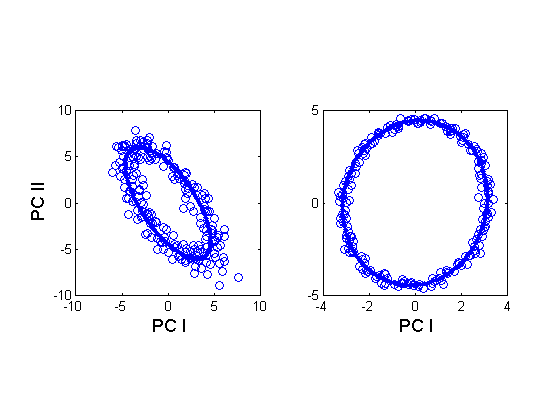
\includegraphics[height=4in, width=6in]{figs/MDA1}
  \caption{The left panel displays estimated factor scores as open circles and the scores used to generate the data as asterisks.  No regularization was used for this analysis.  The right panel shows estimated scores when the column roughness was defined by the projection of scores on to the complement of the space spanned by the true scores, using $\lambda_2 = 10.$}
  \label{MDA1}
\end{figure}
%%%%%%%%%%%%%%%%%%%%%%%%%%%%%%%%%%%%%%%%%%%%%%%%%%%%%%%%%%%%%%%%%

Next we set the column roughness penalty matrix for the estimate of $\Fbold$ to $\Sbold = \Ibold_N - \Fbold_{pop} (\Fbold_{pop}' \Fbold_{pop})^{-1} \Fbold_{pop}'$.  That is, we asked that the factor score estimates fall within the same subspace as is spanned by the two columns of its true counterpart.  This, of course, does not force the estimate to be circular or constrain its orientation if it is not.  The right panel Figure \ref{MDA1} shows the result of using a smoothing parameter $\lambda_2 = 10$ for this penalty.  We see that the estimated scores now correspond more closely to a linear transformation of the true values.  The two squared canonical correlations are now 0.99986 and 0.99808, still indicating a fine subspace recovery; and the values of $H(\Abold)$ were 135.2 and 184.3 for the unregularized and regularized fits, respectively.

%  -------------------------------------------------------------------------------------------

\subsection{Partial least squares variance components}
\label{subsec:MVAPLS}

Estimating a $K$- dimensional subspace of the space of dimension $n$ spanned by the columns of $\Xbold$ can be generalized in many ways.  Partial least squares regression (PLS) estimates a subspace of dimension $K$ within which the approximation of an external set of data in $N$ by $m$ matrix $\Ybold$ is optimal in a least squares sense.  PLS has been found to be preferable to principal components regression in situations where a substantial number of nearly multicollinear covariates are available, and where it considered likely that there is important explanatory variation in the complement of the PCA subspace.  PLS has been found to be especially in chemical engineering and chemometrics where the goal is often to locate compounds imaged in some type of spectrum that play an important role in predicting continuous or classification outcomes.

The term ``partial least squares'' is usually identified with an algorithm developed by H. Wold (1975) and S. Wold (1976) that estimates such an approximation for a dependent vector $\ybold$ through $K$ pairs of weighted averages followed by a deflation of an iterated approximation of $\Xbold$:
\begin{eqnarray} \label{PLSeqtns}
  \pbold^{(k)}   & = & \Xbold^{(k)'} \tbold^{(k)} / \|\tbold^{(k)}\|^2 \nonumber \\
  \tbold^{(k)}   & = & \Xbold^{(k)} (\Xbold^{(k)'} \ybold)             \nonumber \\
  \Xbold^{(k+1)} & = & \Xbold^{(k)'} - \tbold^{(k)} \pbold^{(k)'}, k=1, \ldots, K.
\end{eqnarray}
These iterations are initialized by $\Xbold^{(1)} = \Xbold$ and $\tbold^{(1)} = \Xbold^{(1)} (\Xbold^{(1)'} \ybold) / \|\Xbold^{(1)'}\ybold \|.$  In spite of its simple structure, the algorithm has performed well enough in applications to ensure its incorporation into a wide range of software environments, including Matlab and R.  However, there is no assurance in the algorithm's design that the subspace spanned by $[\tbold^{(1)}, \ldots, \tbold^{(K)}]$ provides an optimal approximation of $\ybold.$

Keeping within the least squares framework and functional relationship (\ref{Feqtn0}), we generalize fitting criterion (\ref{Heqtn1}) using the approach of de Jong and Kiers (1992) as follows:
\begin{equation} \label{HPLSeqtn}
  H(\Abold|\Xbold, \Ybold) = (1-\gamma) \|\Xbold - \Fbold(\Abold) \Abold \|^2 + \gamma \| \Ybold' \Qbold(\Abold) \Ybold \|^2.
\end{equation}
where the relaxation parameter $\gamma \in [0,1]$ and
\begin{equation} \label{Qeqtn}
  \Qbold(\Abold) = \Ibold - \Fbold(\Abold) [\Fbold(\Abold)' \Fbold(\Abold)]^{-1} \Fbold(\Abold)'.
\end{equation}
The second term in the criterion measures the extent to which $\Ybold$ is unpredictable from within the subspace defined by the factor loadings in $\Abold.$  The boundary conditions $\gamma = 0$ and $\gamma = 1$ correspond to pure principal components analysis and pure optimal partial least squares, respectively; and the user has the potential to find a compromise between these objectives that satisfies other objectives such as the interpretability of the subspace itself.  For unregularized lease squares estimation, de Jong and Kiers (1992) showed that a minimizing solution can be obtained by the eigenalysis of
\begin{equation} \label{Geqtn}
  \Sbold_\gamma = (1-\gamma) \Xbold \Xbold' + \gamma \Ybold \Ybold'.
\end{equation}

Again we see that this generalization of PCA and PLS is a nonlinear least squares problem indexed by parameter $\Abold$, so that inference methods available for such problems are readily available.

%  -----------------------------------------------------------------------------------------------
%  ------------------------------------------------------------------------------------------

\section{Functional PCA}
\label{sec:fPCA}

Only minor modifications are required for the analysis of functional data, where the matrix $\Xbold$ is replaced by a set of $N$ functions $x_i$ in $N$-vector $\xbold$, and the principal coefficient matrix $\Abold$ becomes the functional $K$-vector  with values $\abold(t)$.  Let $\abold$ be represented by an expansion in terms of $L$ basis functions $\phi_\ell$, so that $\abold(t) = \Cbold \phibold(t)$, with $\Cbold$ being the $L$ by $K$ matrix of coefficients of the expansion.  

In effect, the computation is equivalent to that of a multivariate analysis in coefficient space in the metric $\Wbold = \int \phibold(t) \phibold'(t) dt$  defined by the $\abold$-basis functions and with data $\Xbold = \int \xbold \phibold'(t) dt$; that is, expressions (\ref{Feqtn1}) and (\ref{Feqtn2}) become
\begin{eqnarray} \label{Feqtn3}
  \Fbold(\abold) & = & \Xbold \Abold'(\Abold \Wbold \Abold + \lambda_1 \Rbold_1)^{-1} 
  \nonumber \\
  \Fbold(\abold) & = & [\Ibold_N \otimes (\Cbold' \Wbold \Cbold) + \lambda_1 \Ibold_N \otimes \Rbold_1 + \lambda_2 \Rbold_2 \otimes \Ibold_K + \lambda_{12} \Rbold_{12}]^{-1} \veccom(\Cbold' \Xbold')  .
\end{eqnarray}
The objective function $H$ is now $H(\abold|\xbold) = \|\xbold - \Fbold(\abold) \abold \| ^2 + P_H$ where the norm in the first term is now defined by summing over $i$ and integrating over $t$.

%  ------------------------------------------------------------------------------------------

\subsection{Principal components of the Berkeley growth data accelerations}
\label{subsec:GrowthAccel}

The Berkeley growth data discussed in Ramsay and Silverman (2005) provide a number of interesting functional data analysis problems.  The functional PCA is illustrated here by the analysis over the age range of three to eighteen years of 54 second height derivative curves for females, calculated from carefully tuned strictly monotone smooths of the original discrete data, and displayed in Figure \ref{FemaleAccel}.  

%%%%%%%%%%%%%%%%%%%%%%%%%%%%%%%%%%%%%%%%%%%%%%%%%%%%%%%%%%%%%%%%%%%%%%%%%%%%%%%%%%%%%%%%%%%%%%%
\begin{figure}
  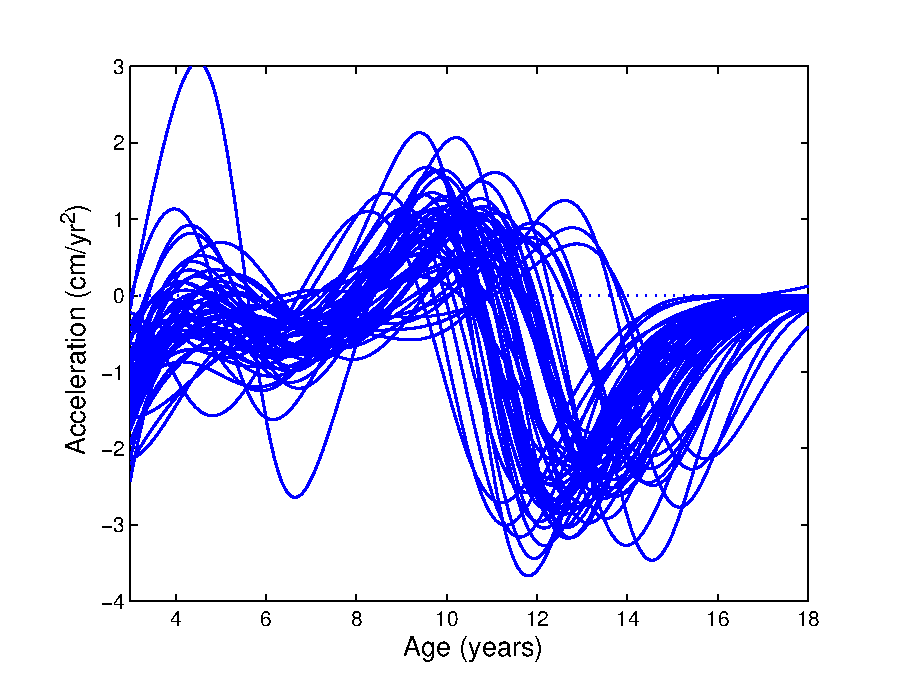
\includegraphics[height=3in, width=5in]{figs/FemaleAccel}
  \caption{The second derivatives of 54 female height curves estimated from the Berkeley growth data, but restricted to begin at three years rather  than the original one year.}
  \label{FemaleAccel}
\end{figure}
%%%%%%%%%%%%%%%%%%%%%%%%%%%%%%%%%%%%%%%%%%%%%%%%%%%%%%%%%%%%%%%%%%%%%%%%%%%%%%%%%%%%%%%%%%%%%%%

In order to reduce computation time, each curve was represented by re-fitting these height accelerations evaluated over 501 equally spaced points using 53 B-spline basis functions with equally spaced knots.  The factor loading functions $\abold$ were represented by 23 B-spline basis functions with equally spaced knots.  The age range was also started at three years rather than one year in order to eliminate the increased instability of acceleration estimates in infancy.  Features to be noted are the wide variation in the age of the middle of the pubertal growth spurt, marked by the crossing of zero with negative slope at around 12 years; and also the single large acceleration variation between three and seven years.

The analyses were first carried out without any regularization for either $\Fbold(\abold)$ or $\abold$; and for $K = 1, \ldots, 4.$  The squared multiple correlations $R^2 = (\SSY - \SSE)/\SSY$, where $\SSY = \sum_i \int x_i^2(t) \, dt$ and $SSE = \sum_i \int [x_i(t) - \fbold_i \abold(t)]^2 \, dt$, for these analyses were 0.683, 0.887, 0.941 and 0.965, respectively; and these values agreed with the corresponding functional principal components values described in Ramsay and Silverman (2005) to four decimal places.  By inspecting the root mean squared residual functions $\RMSE(t) = \sqrt{N^{-1} \sum_i [x_i(t) - \hat{x}_i(t)]^2}$ for each number of factors, shown in Figure \ref{RMSE_FDA}, we can see what each increase in dimensionality of the subspace contributes to the fit.  Steady improvement occurs over $K = 2,3,4$ at age 4, 10.5 and 16, but rather less improvement is provided for the stable later childhood ages 6 to 9 years.  Much of the improvement after age 10 is no doubt due to the improved capacity of higher dimensional fits to account for the variable age of puberty.

%%%%%%%%%%%%%%%%%%%%%%%%%%%%%%%%%%%%%%%%%%%%%%%%%%%%%%%%%%%%%%%%%%%%%%%%%%%%%%%%%%%%%%%%%%%%%%%
\begin{figure}
  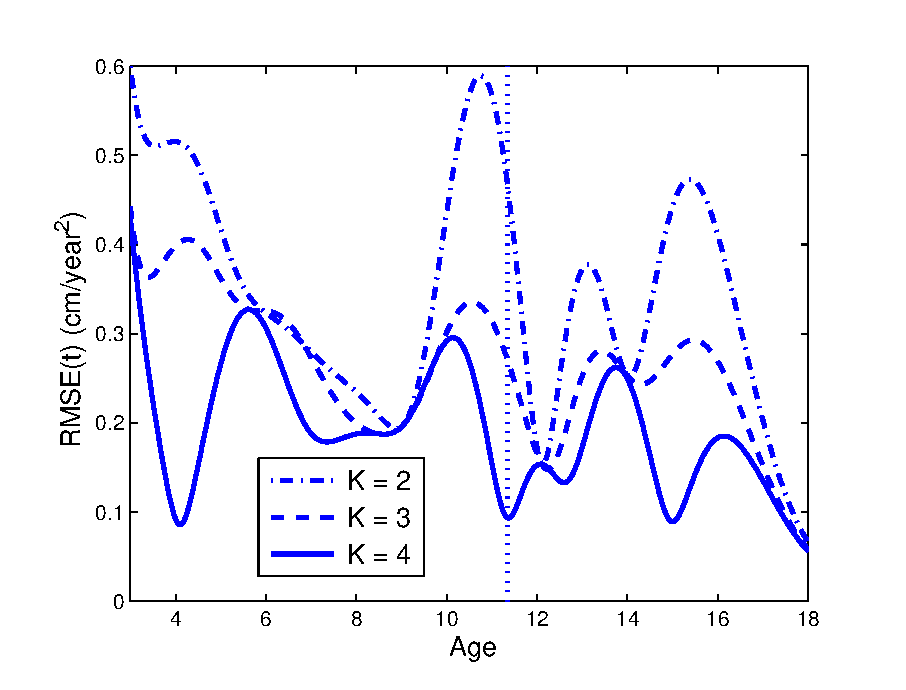
\includegraphics[height=3in, width=5in]{figs/RMSE_FDA}
  \caption{The root mean squared residual for unregistered functional principal component fits to the 54 Berkeley growth acceleration curves for females.  The number of factors ranged from 2 to 4.  The vertical dotted line indicates the average age of middle of the pubertal growth spurt in this sample.}
  \label{RMSE_FDA}
\end{figure}
%%%%%%%%%%%%%%%%%%%%%%%%%%%%%%%%%%%%%%%%%%%%%%%%%%%%%%%%%%%%%%%%%%%%%%%%%%%%%%%%%%%%%%%%%%%%%%%

We then focussed on the two-dimensional PCA in order to consider some regularization.  Figure \ref{GrowthComponent_0} displays the two principal component functions $a_1(t)$ and $a_(2)$ that arise from the unregularized PCA initialized  by the eigenfunctions of the covariance operator computed from the functional data.  As expected, these initial components are already optimal, and no further improvement was achieved by optimizing $H$.  The second component indicated by a dashed line resembles closely the typical shape of an acceleration function, but only accounts for 20\% of the variation.  The dominant component plotted as a solid curve accounts for 67\% of the variance, and acts when added to the second component to shift this component forward or backward in time.  In short, the dominant component of variation in these curves is essentially phase variation, percentage that it represents is close to that given in Kneip and Ramsay (2008).  

%%%%%%%%%%%%%%%%%%%%%%%%%%%%%%%%%%%%%%%%%%%%%%%%%%%%%%%%%%%%%%%%%%%%%%%%%%%%%%%%%%%%%%%%%%%%%%%
\begin{figure}
  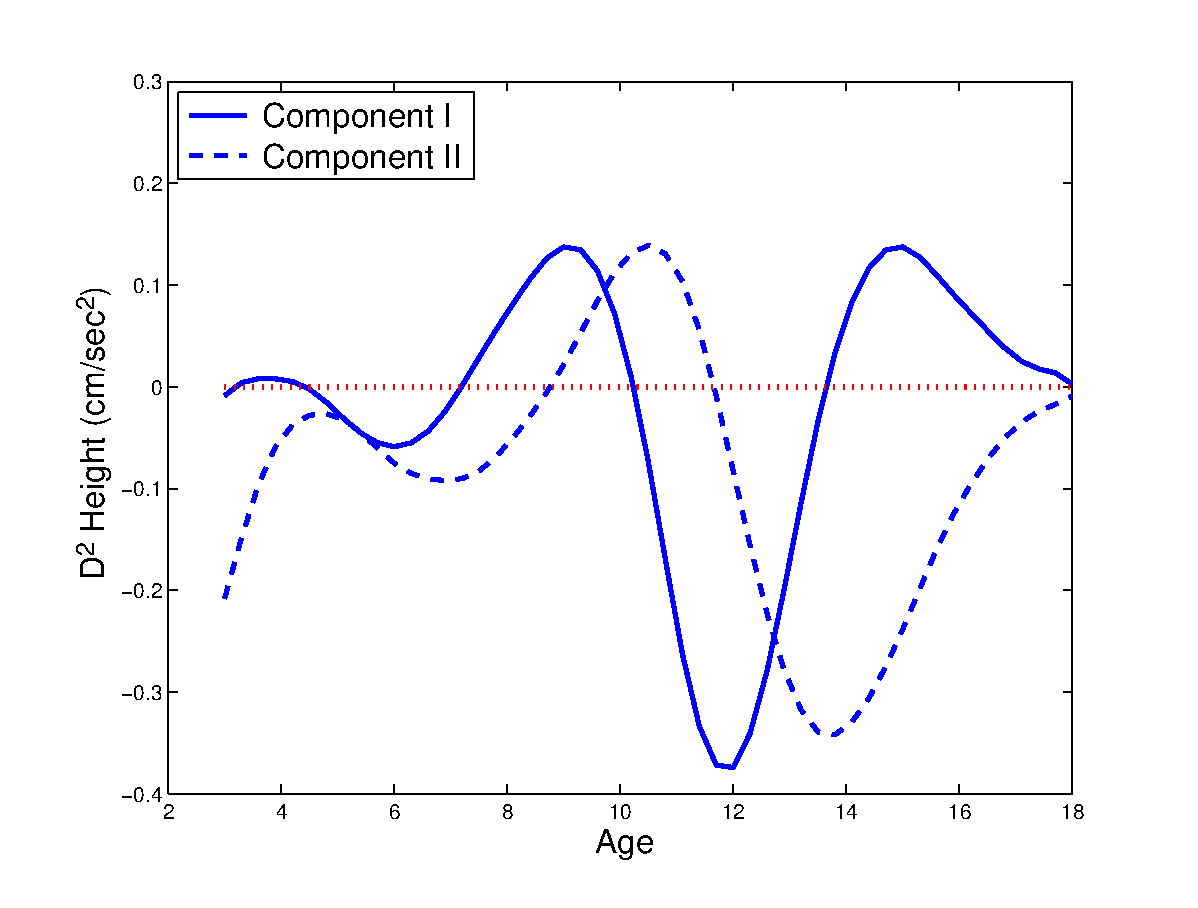
\includegraphics[height=3in, width=5in]{figs/GrowthComponent_0}
  \caption{The first two principal component functions for an unregularized functional PCA of the growth acceleration functions in Figure \ref{FemaleAccel}.  The solid and dashed lines corrrespond to principal components representing 67\% and 20\% of the variation in the original data.}
  \label{GrowthComponent_0}
\end{figure}
%%%%%%%%%%%%%%%%%%%%%%%%%%%%%%%%%%%%%%%%%%%%%%%%%%%%%%%%%%%%%%%%%%%%%%%%%%%%%%%%%%%%%%%%%%%%%%%

The factor scores associated with the unregularized PCA are shown in Figure \ref{GrowthScores}.  We see that these scores tend to be approximately distributed along the segment of a circle with center at the origin.  Figure \ref{GrowthFSmooth} plots the distances of the scores from this origin against the angle of their relations to the origin.  We see that there is an evident descending trend.  This arises because the distances from the origin represent the intensities of the growth spurts, and the angles are associated with how late the pubertal spurt occurs.  Early spurts are intense so as to compensate for a few years to lost growth, while late spurts are mild because more prior growth has already occurred.  The Figure also shows a smoothing spline approximation of this trend, and the arc plotted in the left panel Figure \ref{GrowthScores} is constructed from this smooth.

We now consider a regularization of the PCA.  We use the second term in (\ref{Feqtn3}) to smooth the columns of $\Fbold$ toward the columns of the smooth approximation resulting from converting polar coordinate angle/distance pairs into Cartesian coordinates.  The roughness penalty matrix $\Rbold_2$ projects the columns of $\Fbold$ on to the complement of the space spanned by the columns of this smooth approximation to $\Fbold$.  The right panel of Figure \ref{GrowthScores} displays the result of a rather heavy-handed smoothing using $\lambda_2 = 100$, and we see that the scores now are distributed almost exactly on the approximation.  It is interesting to consider how much this affects the fit to the data;  the error sum of squares increases from 127.2 for the unregularized analysis to 144.7 for this heavy regularized.  The associated squared multiple correlation is $R^2 = 0.12$.  If consider that the right panel is associated with a pure phase variation model, then this again suggests that only about 12\% of the variation in the data is due to amplitude variation in the dashed curved display in Figure \ref{GrowthComponent_0}.  Of course, more principal components increase this percentage, but only slightly it turns out.

%%%%%%%%%%%%%%%%%%%%%%%%%%%%%%%%%%%%%%%%%%%%%%%%%%%%%%%%%%%%%%%%%%%%%%%%%%%%%%%%%%%%%%%%%%%%%%%
\begin{figure}
  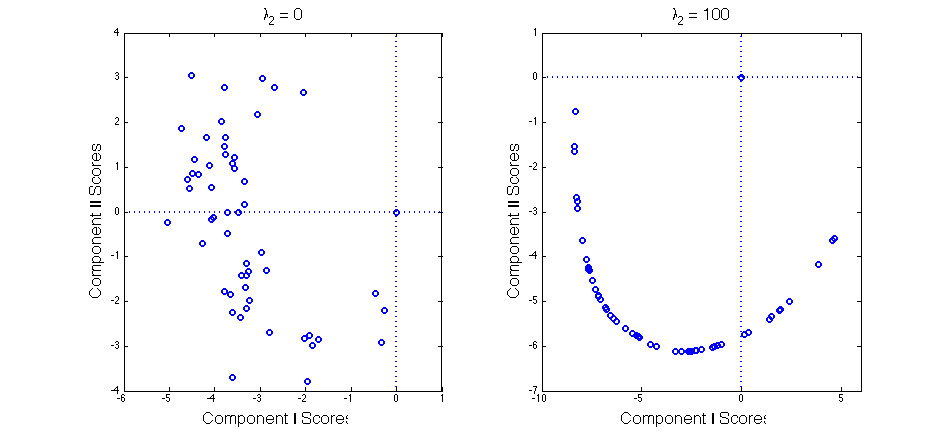
\includegraphics[height=2.5in, width=6in]{figs/GrowthScores}
  \caption{The left panel plots as dots the factor scores derived from an unregularized PCA of the Berkeley growth acceleration curves.  The circles in the right panel define a curved trajectory arising from a heavily regularized PCA result from smoothing the PCA results toward an arc defined by the smooth trend in Figure \ref{GrowthFSmooth}.}
  \label{GrowthScores}
\end{figure}
%%%%%%%%%%%%%%%%%%%%%%%%%%%%%%%%%%%%%%%%%%%%%%%%%%%%%%%%%%%%%%%%%%%%%%%%%%%%%%%%%%%%%%%%%%%%%%%

%%%%%%%%%%%%%%%%%%%%%%%%%%%%%%%%%%%%%%%%%%%%%%%%%%%%%%%%%%%%%%%%%%%%%%%%%%%%%%%%%%%%%%%%%%%%%%%
\begin{figure}
  \includegraphics[height=3in, width=6in]{figs/GrowthFsmooth}
  \caption{The relation of distances from the origin (0,0) of the unregularized factor scores to their corresponding angles from the positive horizontal.  The smooth curve is a function estimated by a smoothing spline with 56 equally spaced knots and a smoothing parameter value of 1.0.}
  \label{GrowthFSmooth}
\end{figure}
%%%%%%%%%%%%%%%%%%%%%%%%%%%%%%%%%%%%%%%%%%%%%%%%%%%%%%%%%%%%%%%%%%%%%%%%%%%%%%%%%%%%%%%%%%%%%%%

%  -------------------------------------------------------------------------------------------

\subsection{Partial least squares for weather data}
\label{subsec:PLSweather}

The weather data described in Ramsay and Silverman (2005) are the context for an interesting comparison of regression on principal components versus the functional version of partial least squares.  In general temperature is primarily of interest as an obvious explanatory variable for a variety of processes that are of more direct interest.  Among these, precipitation is the most important for crop scientists and economies like Canada's that export a large amount of food products.  Here we predict the mean daily precipitation for 35 weather stations, taken over the entire year and over 34 years of observation.

Since the winter months exhibit much more variability, we run the year from July 1 to June 30.  An low-resolution expansion of the daily temperature data averaged over 34 years is shown in Figure \ref{Temperature}.  We attempt to predict mean precipitation in tenths of a millimetre from two functional components which are used to take linear combinations of these 35 curves.  The components PCA and PLS are shown in Figure \label{Daily_PCA_PLS_Components}, and the component scores are displayed in Figure \label{Daily_PCA_PLS_Scores.}  

%%%%%%%%%%%%%%%%%%%%%%%%%%%%%%%%%%%%%%%%%%%%%%%%%%%%%%%%%%%%%%%%%%%%%%%%%%%%%%%%%%%%%%%%%%%%%%%
\begin{figure}
  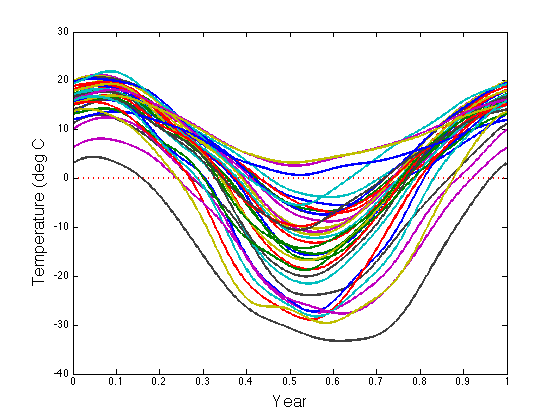
\includegraphics[height=3in, width=6in]{figs/Daily_TempData}
  \caption{Temperature curves for 35 Canadian weather stations over the year beginning July 1 and ending June 30.}
  \label{Temperature}
\end{figure}
%%%%%%%%%%%%%%%%%%%%%%%%%%%%%%%%%%%%%%%%%%%%%%%%%%%%%%%%%%%%%%%%%%%%%%%%%%%%%%%%%%%%%%%%%%%%%%%

%%%%%%%%%%%%%%%%%%%%%%%%%%%%%%%%%%%%%%%%%%%%%%%%%%%%%%%%%%%%%%%%%%%%%%%%%%%%%%%%%%%%%%%%%%%%%%%
\begin{figure}
  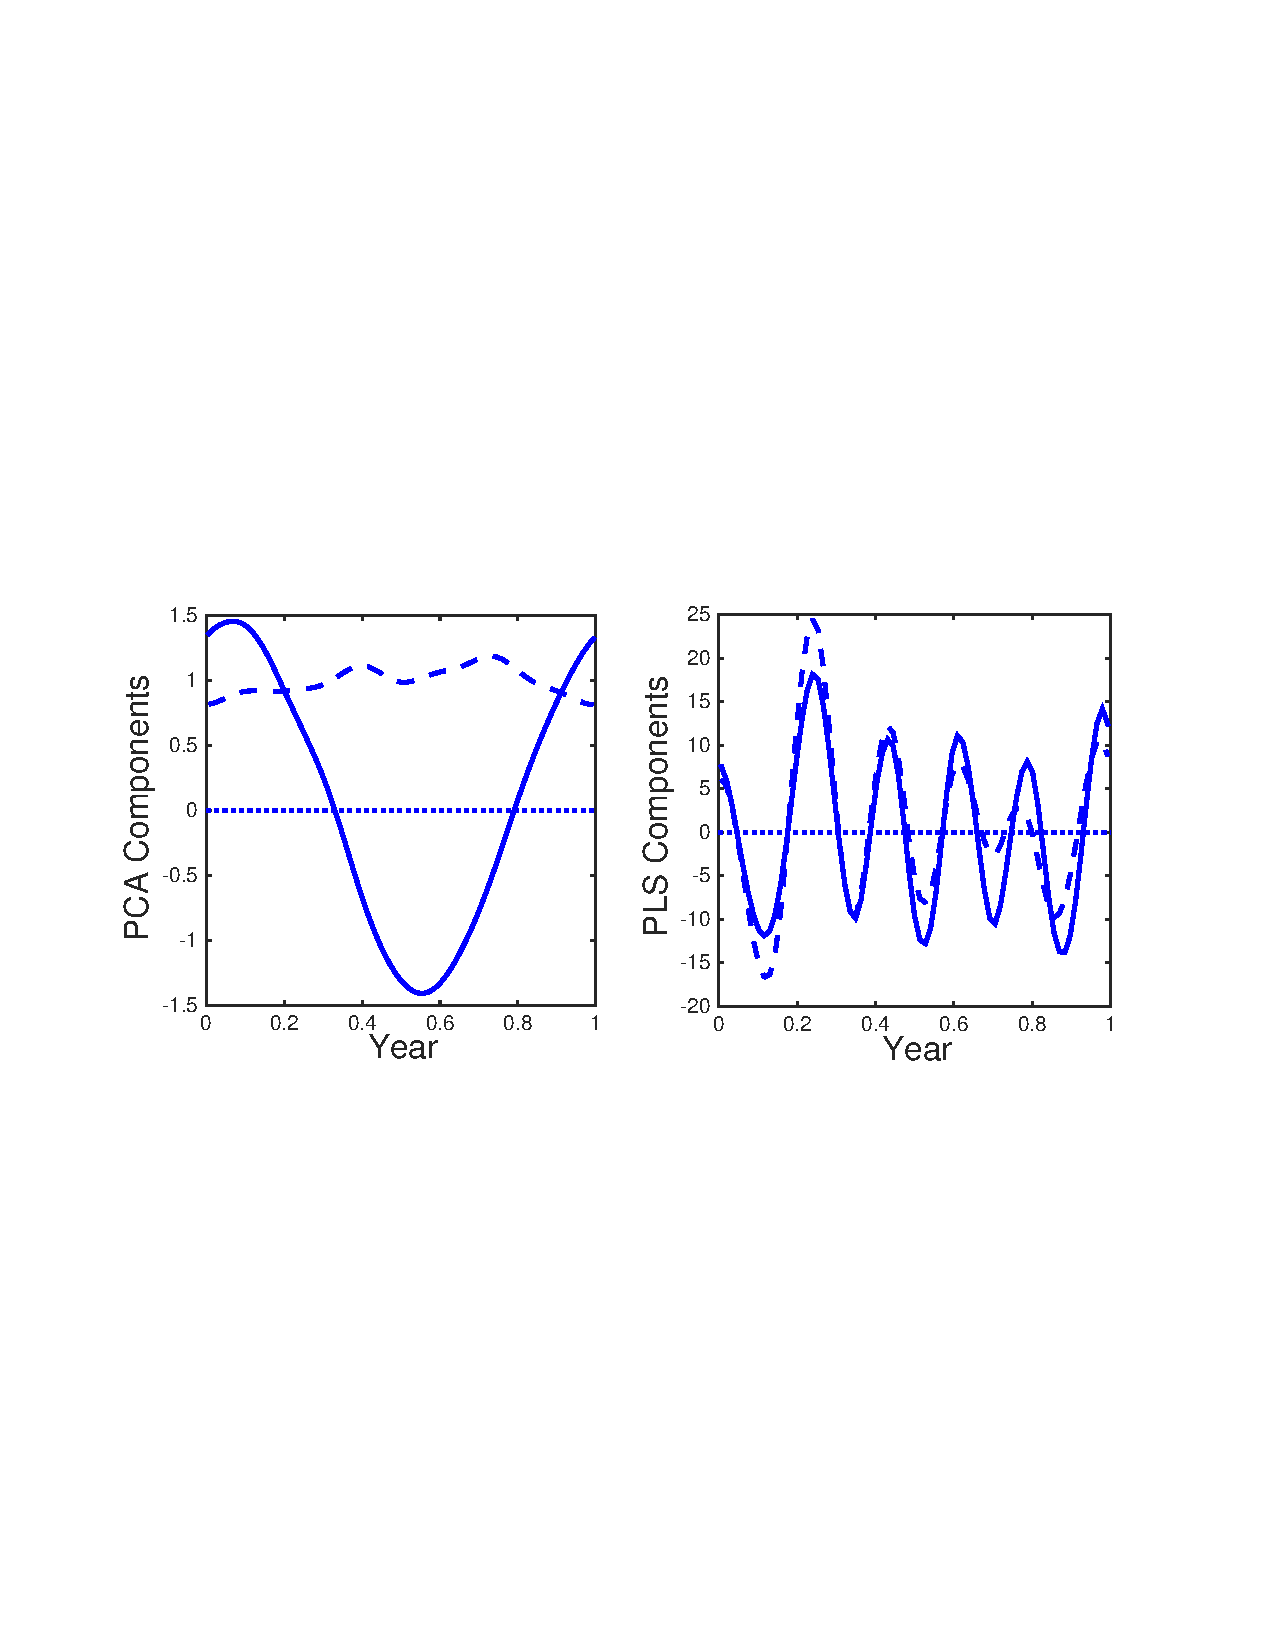
\includegraphics[height=3in, width=6in]{figs/Daily_PCA_PLS_Components}
  \caption{The left panel shows the first two functional principal components for the temperature curves in Figure \label{Temperature} and the right panel shows the two functional components optimizing the fit to the 35 mean precipitations.  In each panel the solid line is the first and dominant component and the dashed line is the subdominant component.}
  \label{Daily_PCA_PLS_Components}
\end{figure}
%%%%%%%%%%%%%%%%%%%%%%%%%%%%%%%%%%%%%%%%%%%%%%%%%%%%%%%%%%%%%%%%%%%%%%%%%%%%%%%%%%%%%%%%%%%%%%%

%%%%%%%%%%%%%%%%%%%%%%%%%%%%%%%%%%%%%%%%%%%%%%%%%%%%%%%%%%%%%%%%%%%%%%%%%%%%%%%%%%%%%%%%%%%%%%%
\begin{figure}
  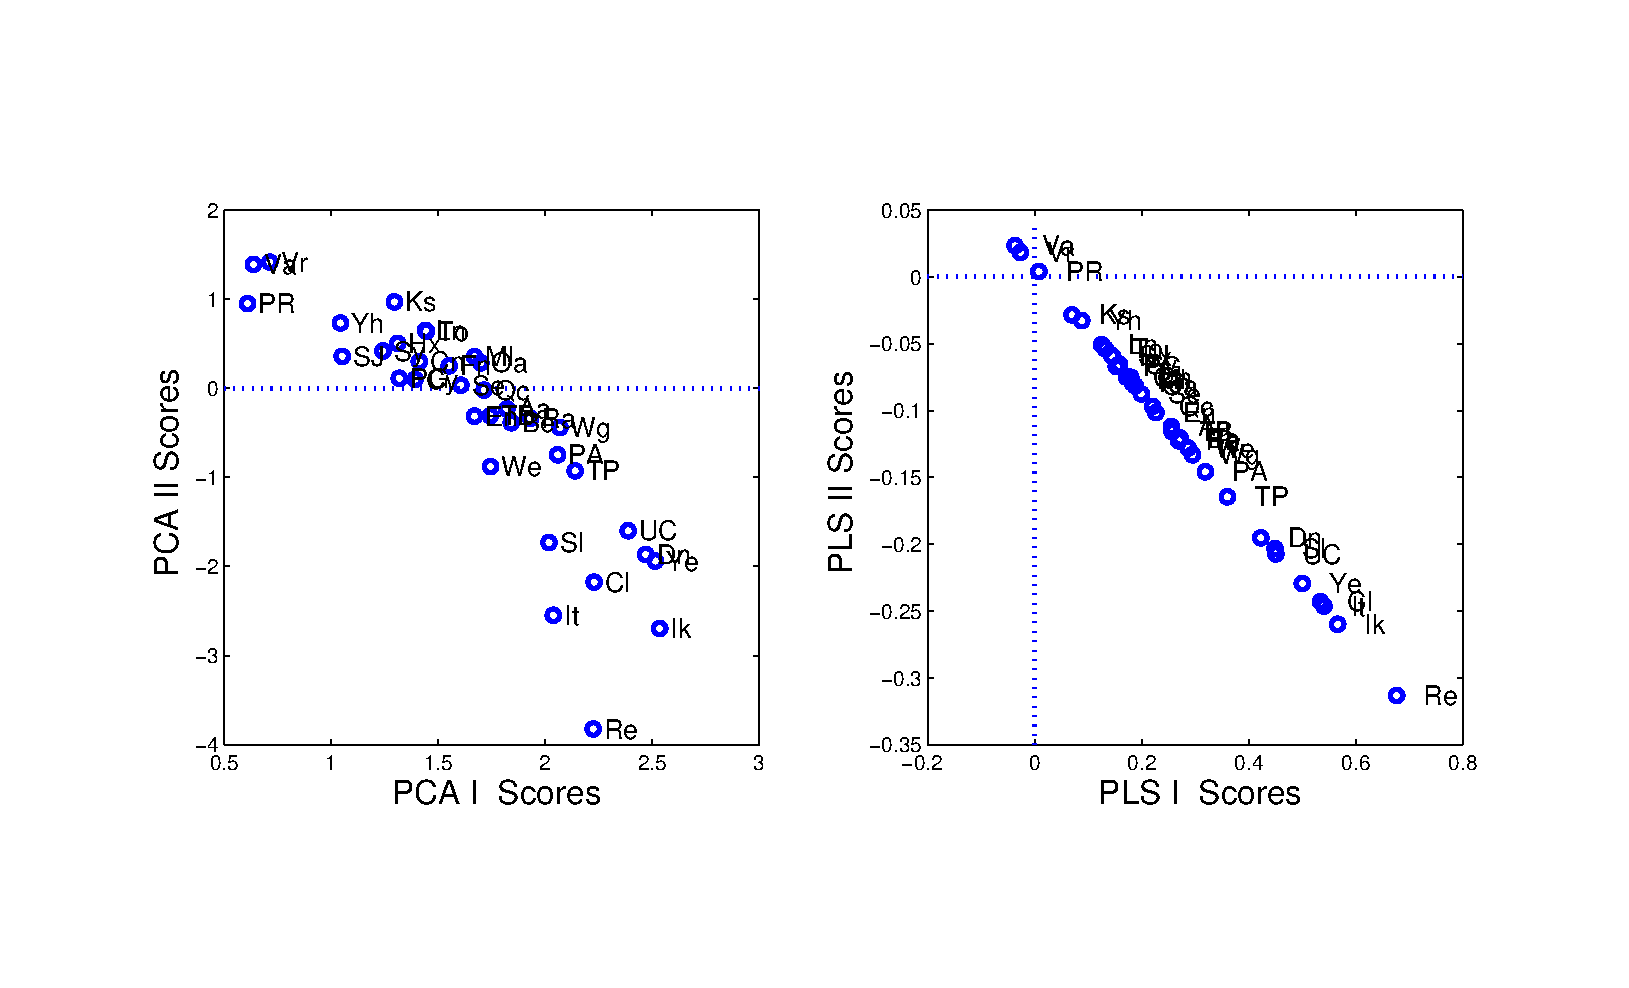
\includegraphics[height=3in, width=6in]{figs/Daily_PCA_PLS_Scores}
  \caption{The left panel shows the first two sets of 35 functional principal component scores for the temperature curves in Figure \label{Temperature} and the right panel shows the functional component scores optimizing the fit to the 35 mean precipitations.}
  \label{Daily_PCA_PLS_Scores}
\end{figure}
%%%%%%%%%%%%%%%%%%%%%%%%%%%%%%%%%%%%%%%%%%%%%%%%%%%%%%%%%%%%%%%%%%%%%%%%%%%%%%%%%%%%%%%%%%%%%%%

The PCA portion of the component plot shows no surprises; the dominant component is mean seasonal variation and the subdominant component is roughly the annual mean temperature.  These two components account for 98.9\% of the variation in the temperature curves.  The corresponding component scores have a mild dispersion around a curved trajectory, with the arctic stations being on the lower right and pacific stations on the upper left. But the PLS components seem to measure something quite different, and the corresponding component scores are virtually linear in their distribution.  Both components have a strong five-cycle periodic shape, with the main difference being in the variation of amplitudes of these cycles across the year.

Figure \ref{Daily_PCA_PLS_Fits} displays the respective fits to the external mean precipitation variable.  The PCA components have a squared multiple correlation of $R^2 = 0.41$, while the PLS components to much better with $R^2 = 0.78.$  Both correlations would be slightly better with the elimination of Prince Rupert, the wettest place in Canada.  We now see five clusters in the PLS fit, corresponding to, going from left to right, arctic, sub-arctic, continental, eastern and Pacific stations, and we see now that the five-cycle pattern in the right panel of the components plot is designed to select out stations in this order.  The time of the year in which this pattern crosses zero with a positive slope can be seen a time of higher slope than is usual for each curve.

%%%%%%%%%%%%%%%%%%%%%%%%%%%%%%%%%%%%%%%%%%%%%%%%%%%%%%%%%%%%%%%%%%%%%%%%%%%%%%%%%%%%%%%%%%%%%%%
\begin{figure}
  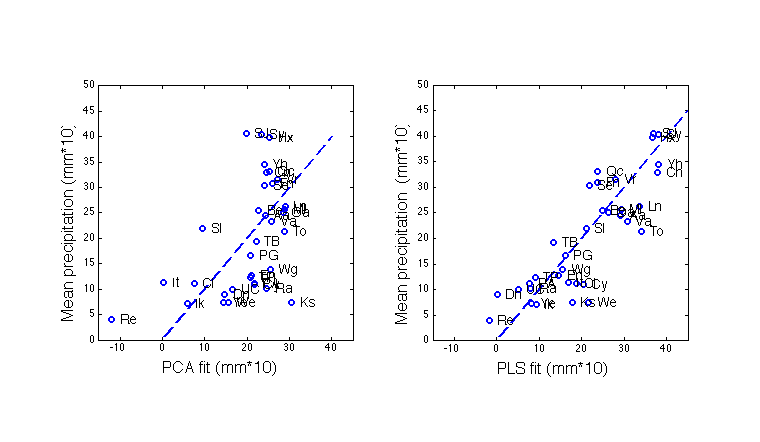
\includegraphics[height=3in, width=6in]{figs/Daily_PCA_PLS_Fit}
  \caption{The left panel shows the approximation of the mean precipitation scores provided by the functional principal component of the temperature curves in Figure \label{Temperature} and the right panel shows the PLS fit to the 35 mean precipitations. Prince Rupert an outlier, and plots above the vertical scale of the plots.}
  \label{Daily_PCA_PLS_Fit}
\end{figure}
%%%%%%%%%%%%%%%%%%%%%%%%%%%%%%%%%%%%%%%%%%%%%%%%%%%%%%%%%%%%%%%%%%%%%%%%%%%%%%%%%%%%%%%%%%%%%%%

Canonical correlation analysis applied to the two score matrices after subtracting their respective column means yields squared correlations of 1.0 and 0.175, indicating that there is a direction in the PCA plane that is unaltered in the PLS counterpart, relative to which the correlation between the respective orthogonal directions is close to zero.

%  -------------------------------------------------------------------------------------------
%  -------------------------------------------------------------------------------------------

\section{Functional PCA with registration}
\label{fPCAReg}

Suppose now that we are in the functional principal component context with $N$ data functions $x_i$; and, as in Section \ref{sec:fPCA}, the $K$ principal components functions $a_k$ define the approximation $\hat{x_i} = \fbold_i(\abold) \abold$.  But now we consider that there is phase variation from one observed function to another, so that instead of measuring time or whatever else $t$ represents on a fixed scale, we need to apply a smooth strictly increasing transformation $\tau_i(t)$ of standard time prior to computing the value of the functions $a_k$ and the factor scores $\fbold_i(\abold)$ that they define.  This case is discussed in detail in Kneip and Ramsay (2008).

A family of a smooth strictly monotonic functions $\tau$ that is defined in terms of a basis function expansion is
\begin{equation} \label{taueqtn}
  \tau(t|\dbold_i') = T \frac{\int_0^t \exp[\dbold_i' \psibold(z)] \, dz }{ \int_0^T \exp[\dbold_i' \psibold(z)] \, dz}
\end{equation}
where $t \in [0,T]$, $\psibold$ is a vector of $M$ basis functions and $\dbold_i$ is a vector of coefficients of length $L$ for the $i$th case defining the basis function expansion in the log of the integrand.  Let $L$ by $N$ matrix $\Dbold$ contain the $\dbold_i$'s in its columns.

The principal component coefficient function for approximating the function value $x_i(t)$ are now $\alphabold[\tau(t|\dbold_i)]$.  Notice that,  according to this notation, each time the coefficients $\Cbold$ are changed, we must revaluate the coefficients $\dbold_i$, so that the time-warping coefficients in $N$ by $M$ matrix $\Dbold$ are themselves functions $\Dbold(\Cbold)$ of structural parameter parameters $\Cbold$, and hence nuisance parameters.  In turn, we also still retain the relation $\Fbold(\abold)$, which now therefore depends on the value of $\Dbold$ as well.  That is, we have a three-level cascade of parameters, indicated by $\Fbold[\Dbold(\Cbold)]$.

The function $\Fbold(\Cbold)$ is no longer linear, as it was in (\ref{Feqtn3}, since it is mediated by what is usually a nonlinear time warping function, such as (\ref{taueqtn}).  In the case of the least squares criterion for $H$, this implies that each time $\Cbold$ is modified in an outer optimization of criterion $H(\Cbold)$, an inner optimization $G(\Dbold|\Cbold)$ is required, which in turn makes use of the linear relation $\Fbold(\abold)$ in (\ref{Feqtn2}).

It is known (Kneip and Ramsay, 2008) that the inner optimization criterion $G(\Dbold|\Cbold)$ ought not to be a least squares measure, since this can produce undesirable estimates of phase variation.  Instead, it has been found quite satisfactory to minimize the smalles--eigenvalue--of--crossproduct criterion (SEofC)
\begin{equation} \label{crossprodmatrix}
    G(\Dbold|\Cbold) = \sum_i^N \MINEIG
  \left[
     \begin{array}{ll}
       \int \{x_i(t)\}^2                          \, dt &
       \int x_i(t) \, \xhat_i[\tau(t|\dbold_i)]   \, dt \\
       \int x_i(t) \, \xhat_i[\tau(t|\dbold_i)]   \, dt &
       \int \{\xhat_i[\tau(t|\dbold_i)]\}^2       \, dt
     \end{array}
   \right] + \lambda_1 \dbold_i' \Vbold \dbold_i.
\end{equation}
The second term in this criterion permits control over the smoothness of the warping functions.  Note that here and elsewhere in the computation inner products of the form $\langle f,g \rangle_\tau = \int (f \circ h)(t) (g \circ h)(t) \, dt.$  See the Appendix for comments on how these may be accurately approximated by the use of a pair of ordinary differential equations.

The principal components analysis of the Berkeley growth accelerations was repeated for $K = 1,2,3$, but this time registering the principal component fit to the functional data.  Seven B-spline basis functions with equally spaced knots were used for the $\psi_\ell$'s, and the integrated squared first derivative roughness penalty was multiplied by a roughness parameter $\lambda_1 = 1.$ The estimated deformation functions $\delta(t) = \tau(t) - t$ for $K=2$ are displayed in Figure \ref{Deform_2}, and we see that the deformations tend to be simple in shape and maximal excursions of about two and half years.  A satellite PCA of the deformation functions reveals only a single large principal component.

%%%%%%%%%%%%%%%%%%%%%%%%%%%%%%%%%%%%%%%%%%%%%%%%%%%%%%%%%%%%%%%%%
\begin{figure}
  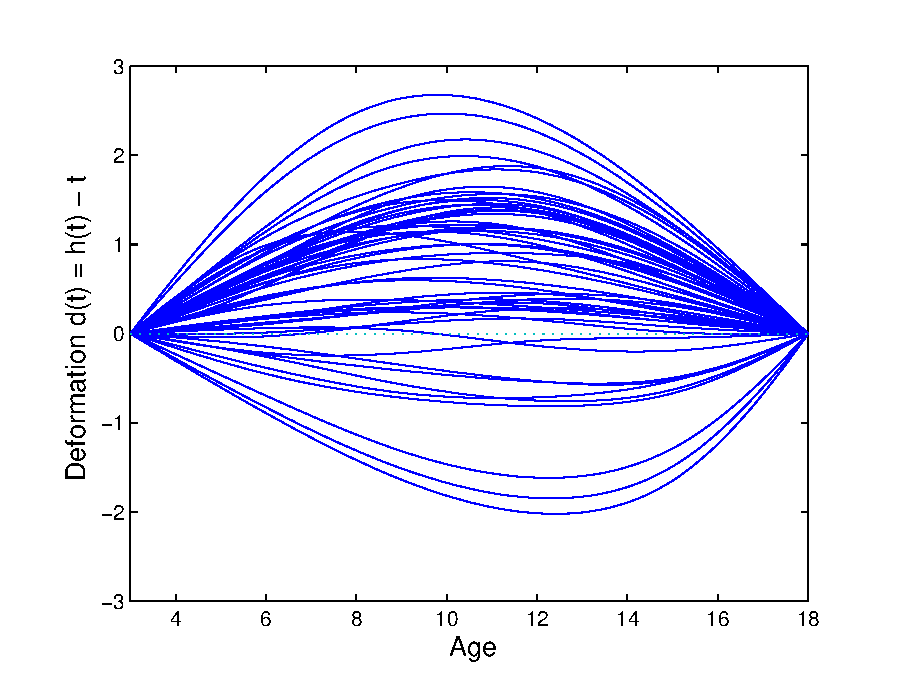
\includegraphics[height=3in, width=5in]{figs/Deform_2}
  \caption{The estimated deformation functions $\delta(t) = \tau(t) - t$}
  \label{Deform_2}
\end{figure}
%%%%%%%%%%%%%%%%%%%%%%%%%%%%%%%%%%%%%%%%%%%%%%%%%%%%%%%%%%%%%%%%%

The squared multiple correlations were 0.924, 0.969 and 0.979, respectively; and these values are each comparable to the corresponding unregistered PCA using two more factors.  Figure \ref{RMSE_Reg} now shows relatively simple increments to fit as $K$ passes from one to three;  The second dimension introduces a factor that accommodates the single large acceleration excursion in early childhood in Figure \ref{FemaleAccel}, and the third factor does a nice job of capturing additional variation in the pubertal growth spurt years that is not due to the timing of the pubertal growth spurt.  In other words, this analysis neatly separates amplitude variation (three dimensional) from phase variation (primarily one-dimensional).

%%%%%%%%%%%%%%%%%%%%%%%%%%%%%%%%%%%%%%%%%%%%%%%%%%%%%%%%%%%%%%%%%
\begin{figure}
  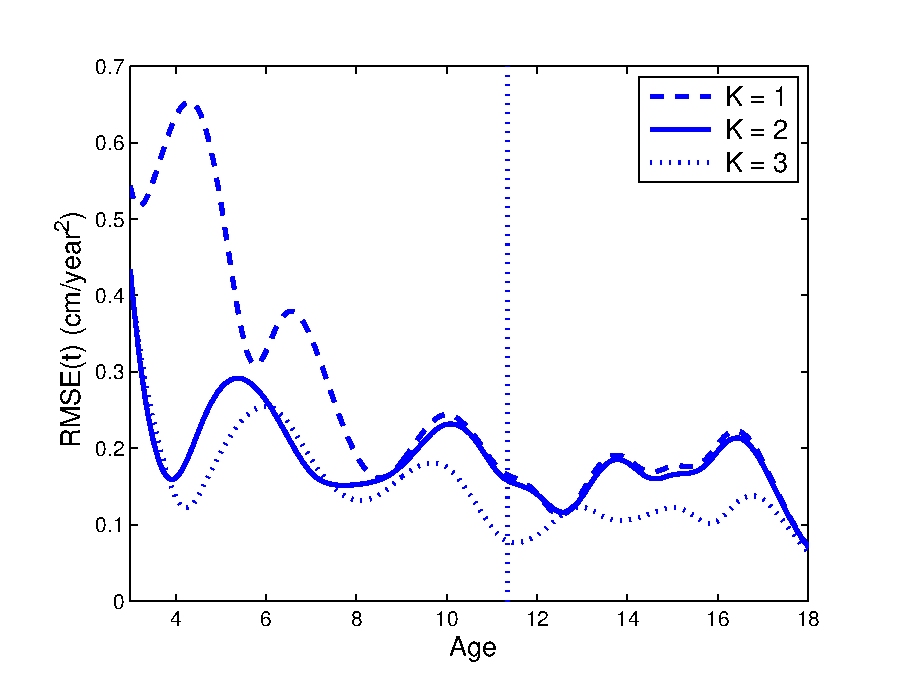
\includegraphics[height=3in, width=5in]{figs/Hfn_Reg_RMSE}
  \caption{The root mean squared residual for registered functional principal component fits to the 54 Berkeley growth acceleration curves for females.  The number of factors ranged from 2 to 4.  The vertical dotted line indicates the average age of middle of the pubertal growth spurt in this sample.}
  \label{RMSE_Reg}
\end{figure}
%%%%%%%%%%%%%%%%%%%%%%%%%%%%%%%%%%%%%%%%%%%%%%%%%%%%%%%%%%%%%%%%%

% -------------------------------------------------------------------------------------------------
%  ------------------------------------------------------------------------------------------------

\newpage

\begin{center}
{\Large Bibliography}
\end{center}

\begin{description}

\item Bates, D. M.  and Watts, D. B. (1988) \emph{Nonlinear Regression Analysis and Its Applications},
    New York: Wiley.

\item Cao, J. and Ramsay, J. O. (2007) Parameter cascades and profiling in functional data analysis. \emph{Computational Statistics,} 22, 335-351.

\item Cao, J. and Ramsay, J. O. (2008) Generalized profiling estimation for global and adaptive penalized spline smoothing. \emph{Computational Statistics and Data Analysis,} 53, 2550-2563.

\item Cao, J. and Ramsay, J. O. (2010) Linear mixed-effects modeling by parameter cascading. \emph{Journal of the American Statistical Association,} 105, 365-374.

\item de Jong, S. and Kiers, H. (1992) Principal covariates regression: Part I. Theory.  \emph{Chemometrics and Intelligent Laboratory Systems,} 14, 155-164.

\item Kneip, A. and Ramsay, J. O. (2008) Combining registration and fitting for functional linear models.  \emph{Journal of the American Statistical Association,} 103, 1155-1165.

\item Neyman, J. and Scott, E. L. (1948) Consistent estimates based on partially consistent observations. \emph{Econometrika,} 16, 1-32.

\item Ramsay, J. O. \& Silverman, B. W. (2005) {\em Functional Data Analysis,} New York: Springer.

\item Ramsay, J. O., Hooker, G., Campbell, D. and Cao, J. (2007) Parameter estimation for differential equations: A generalized profiling approach (with discussion). \emph{Journal of the Royal Statistical Society, Series B,} 69, 741-796.

\end{description}


\end{document}
